% !TEX root = ../main.tex

\chapter{Probabilistic Programming -- the User's Perspective}
\label{chp:probprog}

In this chapter we will provide a high level introduction to probabilistic programming,
outlining its aims and explaining how it can be used for and to extend Bayesian modeling.  The
key points we will covey are the ability of probabilistic programming systems (PPSs) to provide 
the \emph{flexibility} to define
wide ranging and potentially obscure models, the \emph{expressivity} of a framework for 
model definition that is more in line we conventional scientific simulation than mainstream 
statistical approaches, and the \emph{automation} to  run on any problem the user might write
by decoupling model specification and inference.
Together these characteristics produce a framework that allows researchers whose expertise 
lies elsewhere, to carry out powerful statistical analyses and deliver the best possible 
performance for their application specific tasks.  It also aids in the development of both inference
algorithms and models for those within the machine learning and statistics communities,
by removing many of the complications of one while developing the other.

We will for now focus on a user's perspective, introducing how and why one might want to use
probabilistic programming, explain how ideas from more mainstream Bayesian
modeling can be transfered, and demonstrate how probabilistic programming can be
used to both extend the traditional Bayesian framework and reinterpret many computational simulation
techniques not usually associated with Bayesian modeling in a more Bayesian mindset.
We will mostly ignore the rather major issue of how to conduct Bayesian inference for
models defined in probabilistic programs, assuming for now that we have magical
general purpose inference engines that will solve any model we provide,
before returning to actually confront this major stumbling
block in Chapter~\ref{chp:proginf}, once we have introduced the problems of Bayesian
inference more generally.  We will provide a brief introduction to the Anglican PPS
to give us a platform for providing examples and highlighting
key components of designing a PPS.  Finally, we discuss some of the current limitations
and opportunities for PPSs (other than the obvious computational
issues we which return to later), in particular demonstrating how we can use them to go beyond
standard inference frameworks and why we would want to do so.

% !TEX root = ../main.tex

\section{Inverting Simulators}
\label{sec:probprog:inv}

Though the use of Bayesian modeling through the sciences and engineering is widespread,
it is still dwarfed by the use of simulators more generally.  Some simulations are inherently
probabilistic, such as many of those used in statistical physics~\citep{landau2014guide},
 financial modeling~\citep{jackel2002monte}, and weather prediction~\citep{evensen1994sequential}.  
 Others are deterministic approximations
of a truly stochastic world, such as lap time simulation for formula one cars~\citep{perantoni2014optimal}
and finite element simulations for fluid dynamics~\citep{versteeg2007introduction}.
In many of these scenarios, real data is also available, but not in sufficient quantities that the carefully
constructed simulations can be done away with entirely and replaced by a purely data driven
approach.  
Imagine the potential utility of general purpose methods for incorporating real data
into these simulators to improve them, without having to throw away the existing carefully constructed models.  
What about if we could even find methods for automatically
inverting these simulators?  Given a target lap time, we could return the best car setup; given observations
of, and a simulator for, human behavior, we could learn about the underlying cognitive processes; given
a climate change model and measurements, we might infer what the driving factors are.  

An ambitious long
term aim of probabilistic programming is to solve such problems and to do so in an automated fashion
so that it requires little or no statistical expertise on the behalf of the user, allowing for simple, widespread usage
across many fields.  The key realization is that stochastic simulators implicitly define probability distributions.
They, therefore, represent generative models and using probabilistic programming we can reason about, and
work with, these generative models explicitly.  One typically thinks of Bayesian modeling in terms of the
prior and the posterior, but one can also think about it in terms of defining a joint distribution over
both parameters and data, then fixing the latter to the actual observations to get a conditional distribution from
this joint.  Simulators implicitly define such joint distributions, with the outputs of the simulator corresponding
to the data, and the inputs and internal variables the parameters.  Probabilistic programming allows us to turn this on its head,
using the same code as the original simulator, but instead providing the observed data as the input and
then inverting the simulator through inference to learn about possible input parameters and other 
variables sampled during the program's forward execution.  
As well as the clear direct utility of allowing such inversion, this process also allows us to improve
our simulator using real data, by calculating the posterior predictive distribution that incorporates both
the original model and the information from the data.

To explain what we mean by inverting simulators more precisely, we will now consider
the example of inferring Captchas~\citep{mansinghka2013approximate}.   Even if the name is not familiar, 
everyone should hopefully have come across Captchas before when a website shows us an image, such
as those in in Figure~\ref{fig:probprog:example_captchas}, and asks us to
type the characters in that image to demonstrate we are not a robot.  We now ask the
question: how might we write an algorithm that breaks this Captcha by 
automatically predicting these characters directly from the image? In other words, 
can we build a robot that mimics a human on a task specifically designed to 
distinguish between the two.  If we had access to large supply of training examples, i.e.
character-image pairs, we could of course use an off-the-shelf discriminative algorithm:
neural networks have been used to try and solve the problem in exactly this way with reasonable
success~\citep{von2008recaptcha}.  However, without access to an abundance of data this is a rather
challenging task and we will need to exploit our prior knowledge about the problem.  

\begin{figure}[t]
	\centering 
	\begin{subfigure}[t]{0.58\textwidth}
		\centering
			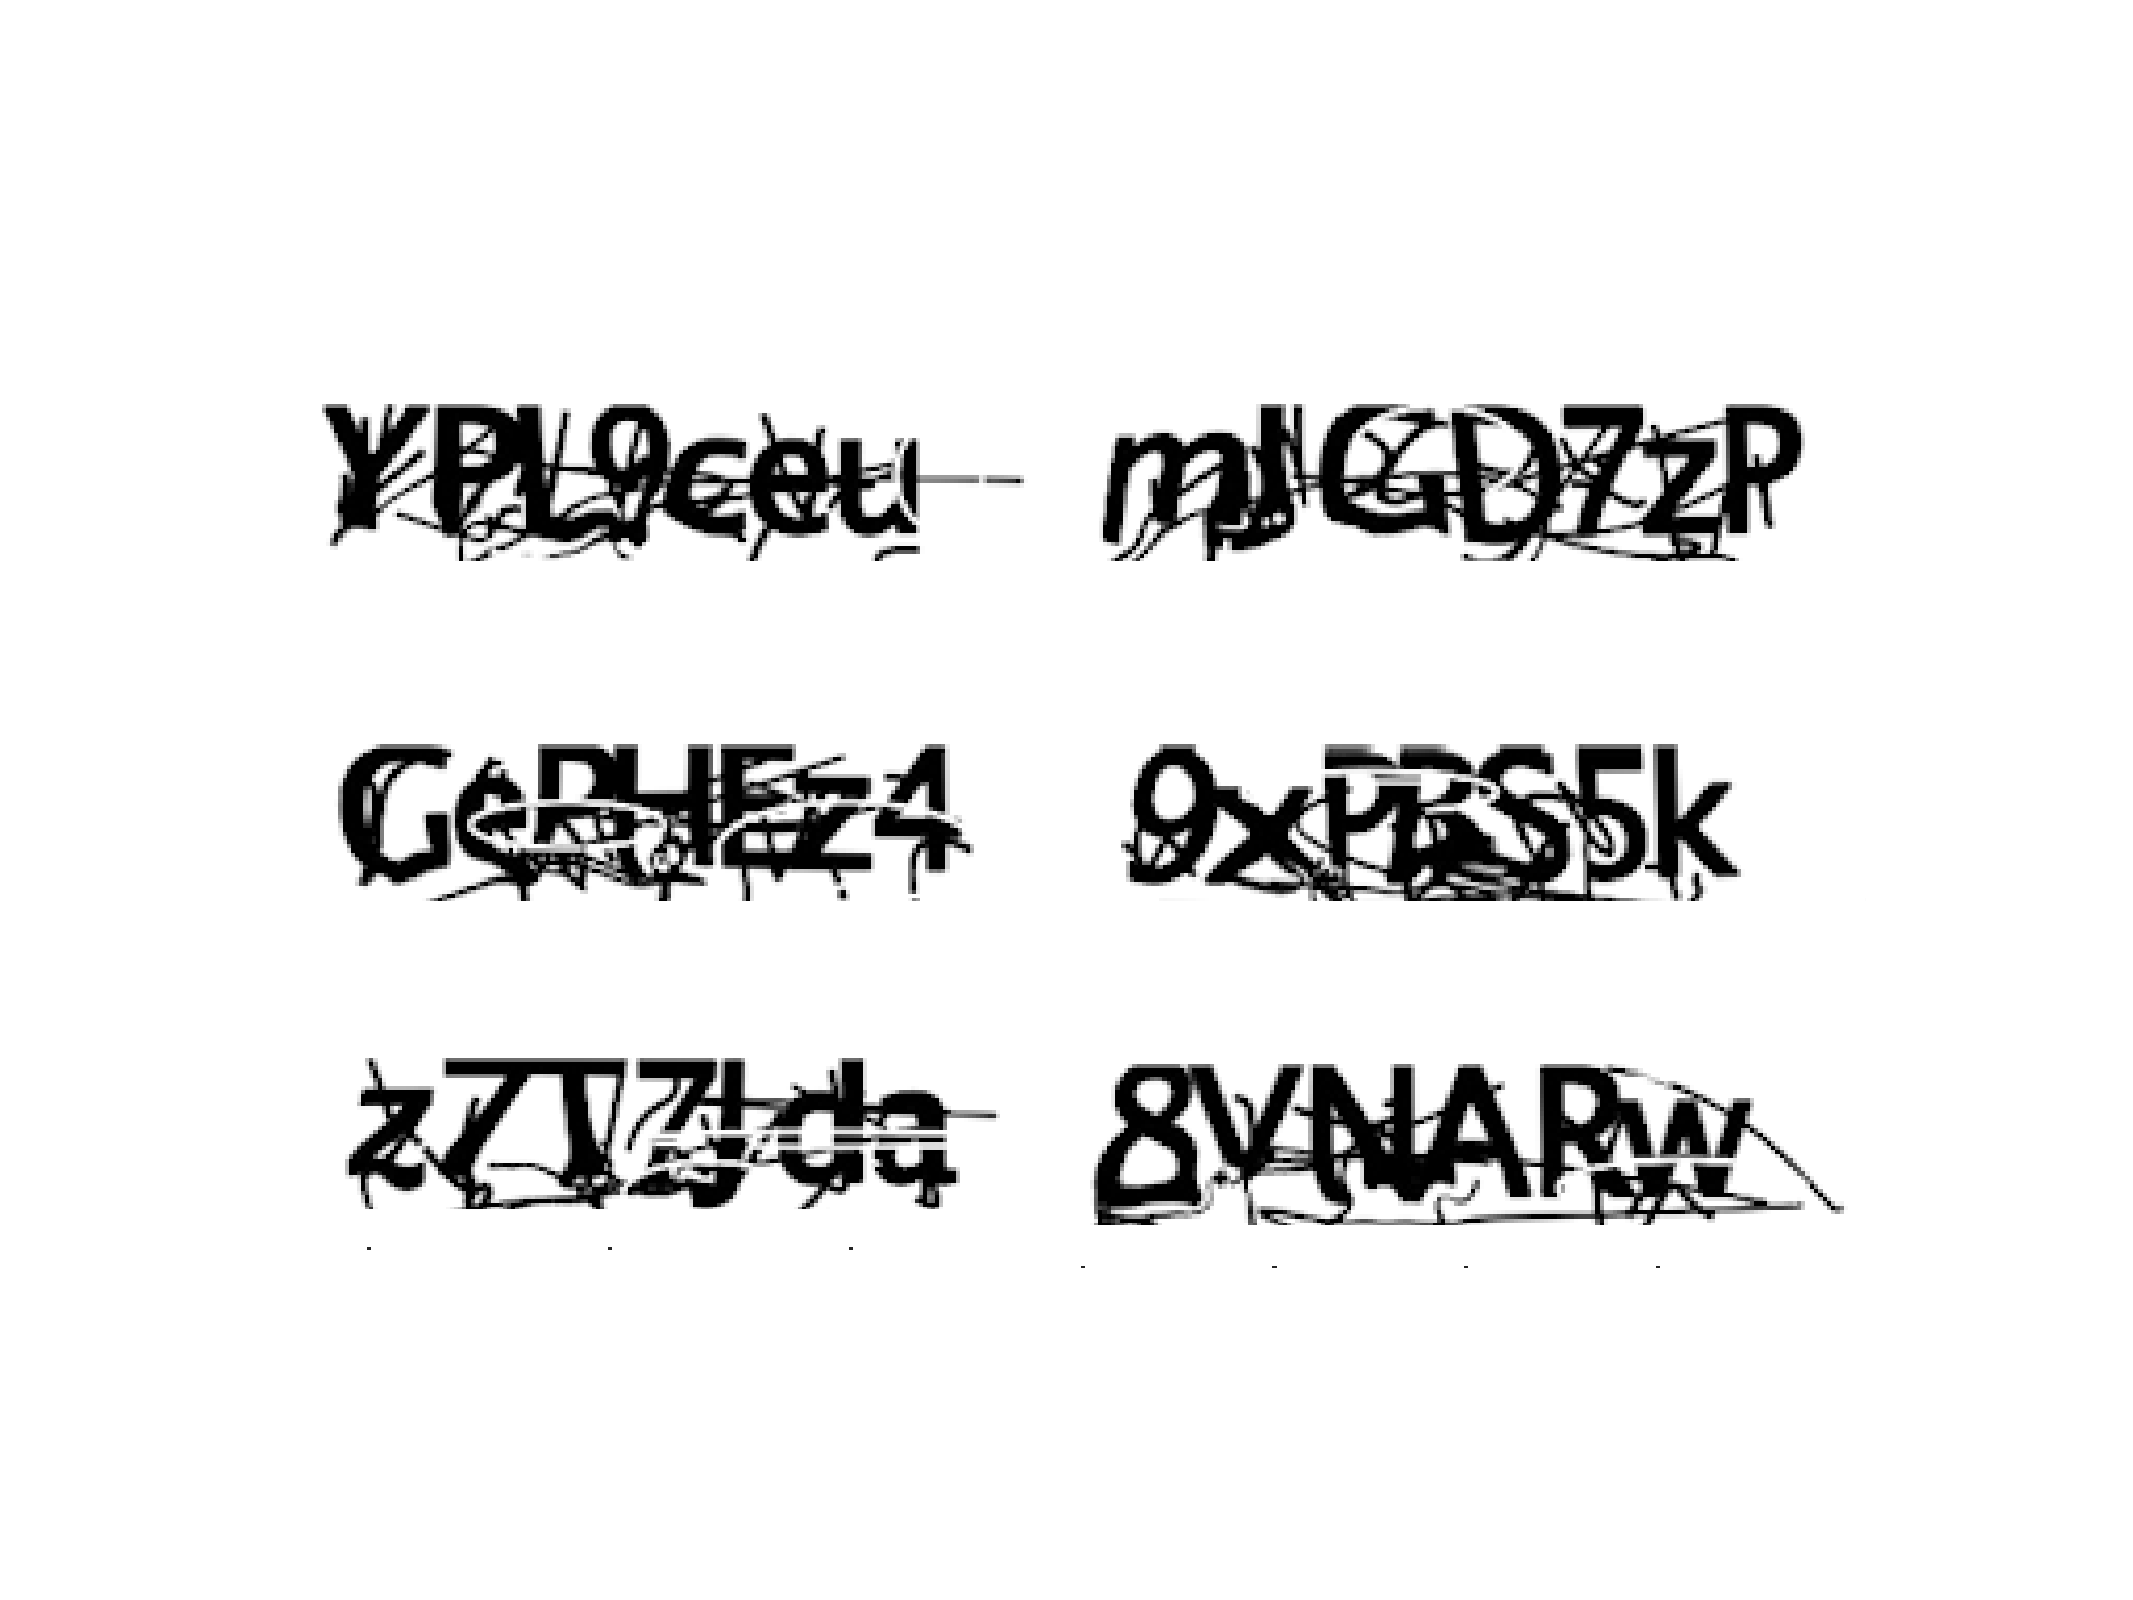
\includegraphics[width=\textwidth]{probprog/figures/example_captchas.pdf}
		\caption{Examples of real Captchas
			 \label{fig:probprog:example_captchas}}
	\end{subfigure}
	~~
	\begin{subfigure}[t]{0.38\textwidth}
		\centering
			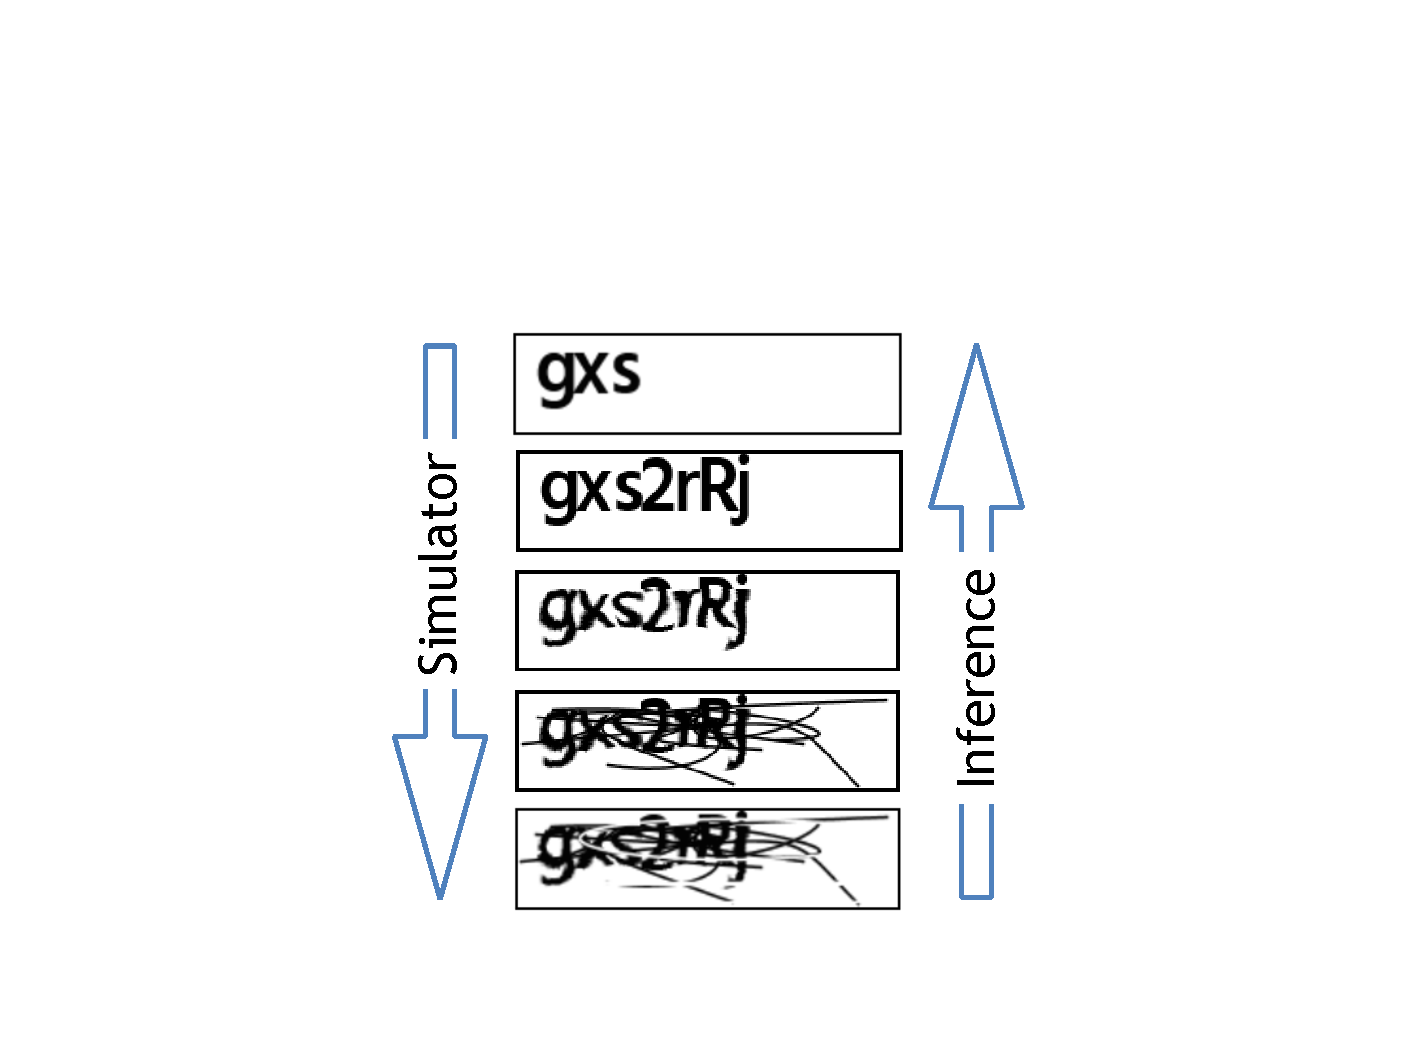
\includegraphics[width=\textwidth]{probprog/figures/captcha_sim.pdf}
		\caption{Example simulation of a Captcha
			\label{fig:probprog:captcha_sim}}
	\end{subfigure}
	\vspace{5pt}
	\caption{Solving Captchas by simulator inversion.   \textbf{(a)} gives examples of real
		Facebook Captchas taken from~\cite{le2017using}.  Here the corresponding
		generating strings going
		to clockwise from the top left are YPL9ceu, mJGD7zP, 9xPBS5k, 8VNARw, z7T7Jda, and
		GePHEz4.  A user is asked to type in these strings when shown the corresponding
		image to show they are not a robot.
		\textbf{(b)} gives an example of the process of simulating Captchas taken by
		~\cite{le2017inference}.  Here we see that we can generate a Captcha by first
		simulating a series of characters, then simulating appropriate manipulations 
		to those characters such as warping, rotating, and adding noise.  Inverting this
		simulation process corresponds to an inference problem, where we want to find
		out the characters that lead to a particular image.
		\label{fig:probprog:captcha}}
\end{figure}

Doing this process in reverse, i.e. simulating a Captcha, on the other hand, is a substantially
less daunting process.  The true Captchas are actually generated by
a simulator and so we can attempt to mimic this original simulation process.
For example, as shown in Figure~\ref{fig:probprog:captcha_sim} we might first sample a 
number of characters, then a symbol for each character, apply manipulations such as rotations and warpings, simulate
some obscuring lines or other noise, and finally render our simulated components into an
image.  Though admittedly it might take some time and effort to construct a high fidelity
simulator that well matches the produced images, the technical requirements for doing this
(other than possibly the final rendering) are minimal and so it could be carried out by most
people with a reasonable degree of experience in scientific programming.  The number of
people able to write such a simulator should certainly be substantially larger than the
number of people with sufficient experience in Bayesian modeling to construct an equivalent
graphical model or direct mathematical formulation.  The number of people
with the expertise to then write an appropriate inference scheme for the problem is even
smaller.  In a PPS, writing this simulator and providing the data is all that is required.
Given these, the PPS will carry out the inference required to invert the simulator automatically,
inferring the characters from the image.  More generally, we are estimating the inputs and
internal variables of our simulator, given target values for the outputs.

There are two key factors to realizing our aim of inverting simulators.  Firstly we need to provide a 
language which easily allows users to
write down simulators and which has semantics that allows the compiler to extract an appropriate
representation of the joint distribution.  In other words, we need our language to be sufficiently
general purpose and easy to use to not burden the user, while at the same time having syntax and semantics that
ensure the corresponding joint distribution is well defined and can be converted into a form where
we can run inference.  Doing this will require the introduction of means for \emph{conditioning} on data
and of specially defined \emph{random primitives} whose behavior can be controlled at 
run time, rather than just always sampling from
the same predefined distribution as they would in an ordinary programming language.  
The latter can be thought of as defining terms in the prior and the
former as terms in the likelihood as we will discuss in Section~\ref{sec:probprog:models}.
For certain cases, one can alternatively think of conditioning as applying \emph{constraints} to the
program.  For example, we can think of a probabilistic program as defining a simulator
and a set constraints that must be satisfied; this is exactly
how the PPS Church~\citep{goodman2008church} is designed.  An important distinction 
here though is between \emph{hard} and \emph{soft} conditioning.  Hard conditioning is as per the conventional
interpretation of a constraint -- we condition on the fact that an event occurs exactly.  Soft conditioning instead
assigns a weight to the program based on the probability (or probability density) of a given event occurring.
Though hard conditioning is a particular case of soft conditioning (for which the weight is either 1 or 0),
one can, at least semantically, use it to specify a soft conditioning, say 
$p(Y=y | X=x)$, by sampling $Y\sim p(y|X=x)$ and then imposing the constraint $Y=y$.
However, only supporting hard conditioning in a PPS is somewhat restrictive for practical
use, as one cannot effectively condition on continuous data because there is zero probability of
satisfying the resulting constraint.

The second key factor is that our language needs a general purpose inference(s)
engine capable of working on any program the user writes.  Bayesian models are fully defined
by their joint distribution and the data.  Therefore, once a user has written their simulator and provided
the data, this uniquely defines a posterior and the only problem is in solving the resulting Bayesian inference.
If we can now construct inference engines capable of working on arbitrary code, we can 
automate inference on any simulator or model the user defines, creating an
abstraction barrier between model definition and drawing inferences from that model.  We will discuss how this can be
done at length in Chapter~\ref{chp:proginf}.

If we can construct a system that can successfully carry out these tasks, 
the huge potential applications this could provide should be clear. We would have a 
system where the user requires no expertise in inference or conventional
Bayesian modeling in order to write application specific models and have them solved automatically.
Instead, they need only have the ability to write stochastic simulators for the process they wish to
model, a skill possessed my most of the scientific community and many of those outside it as well.
In a hypothetical future where scientists
code all their simulators in extremely powerful PPSs, tasks such as
inverting those simulators and improving the simulator by incorporating real data would
be automated in the same way current compilers convert high-level coding languages to machine code.  
However, this ability is not completely
hypothetical -- many such problems can already be handled by existing systems.  The challenge
is improving and scaling such systems to deal effectively with more difficult and more wide ranging models
in a tractable manner.  The need for such systems to work in an automated manner for a wide array
of possible problems makes this a very difficult problem; after all we are somewhat flaunting the no-free-lunch
theorem.  However, there is a key component that provides hope that this may be possible: we have access
to the target source code of the simulator itself, rather than needing to treat it as a black-box as is the
case for, say, approximate Bayesian computation (ABC) methods~\citep{csillery2010approximate}.  Therefore
maybe we can have our cake and eat it by using the source code itself to guide our algorithms, such that
they behave in problem specific ways.  We will discuss how this can be done at length in 
Chapters~\ref{chp:proginf} and~\ref{chp:bopp}.

\section{Bayesian Models as Program Code}
\label{sec:probprog:models}


Ability to use implicit measure without defining them.

\section{Two Distinct Approaches}
\label{sec:probprog:two}

Probabilistic programming systems allow users to define probabilistic models using a domain-specific programming language. A probabilistic program implicitly defines a distribution on random variables, whilst the system back-end implements general-purpose inference methods.  

PPSs such as Infer.Net \citep{minka_software_2010} and Stan \citep{carpenter2015stan} can be thought of as defining graphical models or factor graphs.  Our focus will instead be on systems such as Church \citep{goodman_uai_2008}, Venture \citep{mansinghka2014venture}, WebPPL \citep{goodman_book_2014}, and Anglican \citep{wood2014new}, which employ a general-purpose programming language for model specification. In these systems, the set of random variables is dynamically typed, such that it is possible to write programs in which this set differs from execution to execution.  This allows an unspecified number of random variables and incorporation of arbitrary black box deterministic functions, such as was exploited by the \simulatec function in Figure \ref{fig:house-heating-code}. The price for this expressivity is that inference methods must be formulated in such a manner that they are applicable to models where the density function is intractable and can only be evaluated during forwards simulation of the program. 


\section{An Introduction to Anglican}
\label{sec:probprog:anglican}

One such general purpose system, \emph{Anglican}, will be used as a reference in this paper.  In Anglican, models are defined using the inference macro \defquery. These models, which we refer to as queries \citep{goodman_uai_2008}, specify a joint distribution $p(Y,X)$ over data $Y$ and variables $X$. Inference on the model is performed using the macro \doquery, which produces a sequence of approximate samples from the conditional distribution $p(X|Y)$ and, for importance sampling based inference algorithms (e.g. sequential Monte Carlo), a marginal likelihood estimate $p(Y)$.  

Random variables in an Anglican program are specified using \sample statements, which can be thought of as terms in the prior. Conditioning is specified using \observe statements which can be thought of as likelihood terms.  Outputs of the program, taking the form of posterior samples, are indicated by the return values.  There is a finite set of \sample and \observe statements in a program source code, but the number of times each statement is called can vary between executions.  We refer the reader to  \href{http://www.robots.ox.ac.uk/~fwood/anglican/}{\small\url{http://www.robots.ox.ac.uk/~fwood/anglican/}} for more details.

\section{Going Beyond Bayesian Inference}
\label{sec:probprog:limit}
